\chapter{智能的最终结构定义}
\label{chap:intelligence-final-structural-definition}

\begin{chapteroverviewbox}
本章是全书关于“智能是什么”这一根本问题的认识论收束。我们将不再从某一种模型、某一种算法、某一种生物器官或某一种工程实现出发定义智能，而是回到贯穿全书的共同对象：\textbf{结构、表示、闭环、时间尺度、承载、迁移、现实反馈与自我重组}。从最初“智能是具有时空尺度的持续动力学过程”，到 CSO 与 Agent-CSO 的区分，再到认知结构在功能拓扑和时间尺度上的迁移，以及 World--Agent--World 闭环和功能自反性的建立，我们最终得到的不是一个单句式的静态定义，而是一组具有严格包含关系的结构定义。

本章据此确立如下最终命题：\textbf{智能不是单纯的计算能力、信息处理能力或任务求解能力，而是一类能够在有限现实条件下形成关于结构的内部结构，并使这些结构进入预测、选择、行动、学习与自我重组闭环，从而持续改变自身与外部世界未来结构的多尺度自反动力过程。}这一表述并不预设主观意识，也不要求某一种特定材料、神经结构或计算架构；它首先是一项功能动力学定义。凡涉及“宇宙看见自己”“结构理解自身”等表述，均应理解为结构与功能意义上的自表示和自调节，而非未经证明的现象意识断言。
\end{chapteroverviewbox}

\begin{figure}[htbp]
\centering
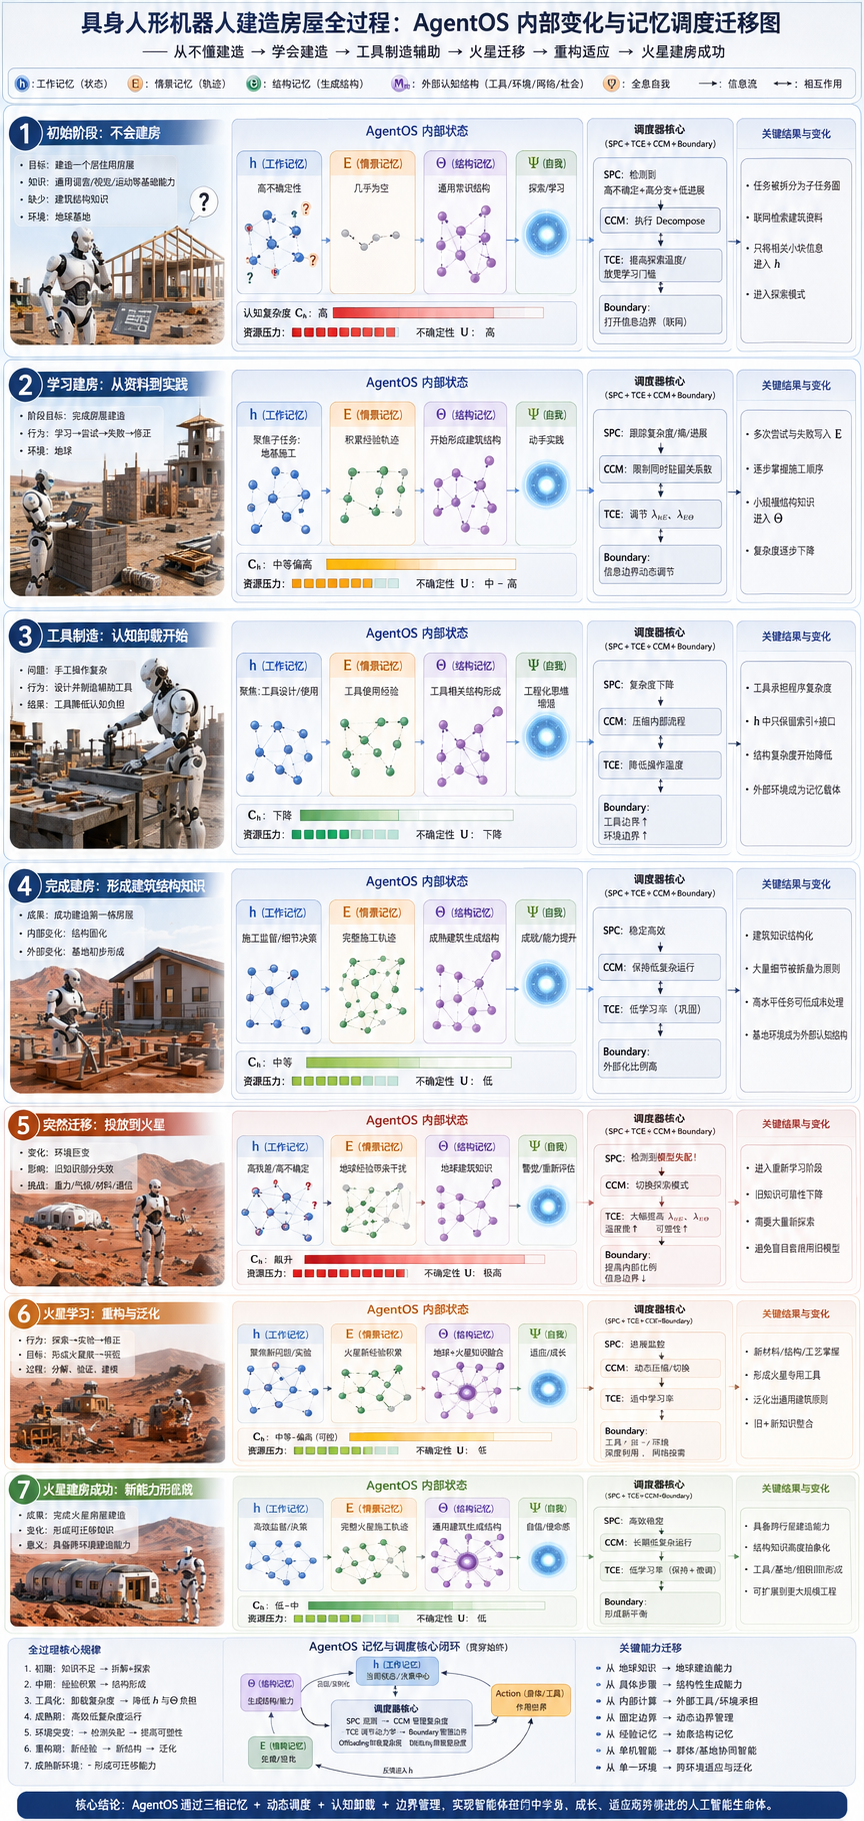
\includegraphics[width=.9\textwidth,height=.38\textheight,keepaspectratio]{images/comparative-intelligence-atlas.png}
\caption{智能作为现实反馈下的跨尺度自反结构过程}
\end{figure}
\begin{introduction}[本章导航]
  \item 多时空尺度上的持续闭环
  \item 认知结构对象的组织、迁移与稳定
  \item 关于结构的结构与未来生成
  \item 现实反馈下的自重组智能
\end{introduction}

\section{从单一定义转向逐层收敛的智能定义体系}

如果我们试图在研究开始时直接回答“什么是智能”，最容易犯的错误就是把某一时代最显眼的技术能力误认为智能本身。符号主义时代可以把智能等同于规则推理，统计学习时代可以把智能等同于函数逼近，大模型时代又很容易把智能等同于语言预测、上下文推理或者参数规模。然而，一旦我们的研究对象从一次性的模型调用扩展为能够经历现实、形成记忆、保持身份、学习技能、改变身体控制方式并在生命周期中持续存在的 Agent，这种以单项能力为中心的定义便迅速失效。我们因此需要的不是另一个更宽泛的能力列表，而是一个能够解释不同智能实现为什么仍属于同一类动力现象的结构定义。

本书最早建立的定义是：

\[
\boxed{
Intelligence
=
MultiscaleClosedLoopProcess
}
\]

即智能首先是一个具有空间边界、时间尺度和闭环结构的持续过程。这里的关键并非“闭环”三个字本身，而是我们拒绝把智能理解成一个脱离时间的静态函数。一个模型在输入 \(x\) 上产生输出 \(y\)：

\[
y=f_{\theta}(x)
\]

只能描述智能系统某一局部映射。如果系统能够持续存在，其真实状态必须写成：

\[
X(t+\Delta t)
=
\Phi
\left(
X(t),
O(t),
A(t),
E(t)
\right),
\]

其中 \(X(t)\) 是智能体当前内部状态，\(O(t)\) 是对现实的观测，\(A(t)\) 是其行动，\(E(t)\) 是现实环境自身的动力状态。于是智能不再是：

\[
Input\rightarrow Output,
\]

而是：

\begin{statementbox}
\centering
\adjustbox{max width=.96\linewidth}{\(\displaystyle World
\rightarrow
Observation
\rightarrow
InternalDynamics
\rightarrow
Action
\rightarrow
World'\)}
\end{statementbox}

这一第一层定义解决了“智能为何具有时间”的问题，却还没有解决一个更深的问题：\textbf{闭环内部究竟有什么东西在发生变化？}

因此第二层定义进入认知结构：

\[
\boxed{
Intelligence
=
CognitiveStructureOrganization
}
\]

在这里，智能不再被描述为抽象信息流，而被描述为 CSO 以及其在特定智能体内部的 Agent-CSO 的生成、激活、组合、压缩、迁移和稳定。一个智能体并不是简单拥有更多数据，而是逐渐建立关于对象、关系、因果、目标、约束、计划、自我和可能未来的结构。我们因此可以把智能内部状态更精确地表示为：

\[
\mathfrak A(t)
=
\left[
\mathcal G_C(t),
\mathcal G_F(t),
\mu_t,
\mathcal M(t)
\right],
\]

其中 \(\mathcal G_C\) 是认知结构图，\(\mathcal G_F\) 是功能拓扑，\(\mu_t\) 描述认知结构在功能拓扑中的动态承载关系，而 \(\mathcal M(t)\) 则表示记忆、自我、目标与当前激活状态等多尺度结构。

然而，即使能够形成复杂内部结构，也仍然不足以区分智能系统与普通复杂动力系统。于是第三层定义出现：

\[
\boxed{
Intelligence
=
StructureThatRepresentsStructure
}
\]

某个结构不仅存在，而且能够在自身内部形成关于另外一个结构的结构。也就是说：

\[
C
\longrightarrow
AgentCSO(C).
\]

当这种表示进一步包含智能体自身：

\[
A
\longrightarrow
AgentCSO(A),
\]

系统便形成了功能意义上的自表示。但是，仅有表示仍然不足以完成最终定义。地图、数据库、录像也能够承载关于现实的结构，却不能因此自动构成完整智能。真正决定智能性质的第四次跃迁，是表示开始参与现实因果：

\begin{statementbox}
\centering
\adjustbox{max width=.96\linewidth}{\(\displaystyle Representation
\rightarrow
Prediction
\rightarrow
Selection
\rightarrow
Action
\rightarrow
RealityChange.\)}
\end{statementbox}

因此第四层定义成为：

\[
\boxed{
Intelligence
=
StructureThatUsesRepresentations
ToTransformFutureStructure
}
\]

最后，当一个系统不仅能够依据表示改变当前行为，而且能够通过长期经验改变生成这些行为的记忆、策略、自我约束、技能位置乃至功能拓扑时，智能才进入本书所称的成熟自反阶段：

\[
\boxed{
Intelligence
=
Representation
+
Control
+
Learning
+
SelfReorganization.
}
\]

我们因此不应在这些定义中选出一个而否定其他定义。它们之间实际上构成严格递进关系：

\begin{statementbox}
\centering
\adjustbox{max width=.96\linewidth}{\(\displaystyle Process
\rightarrow
Structure
\rightarrow
Representation
\rightarrow
RepresentationDrivenAction
\rightarrow
SelfReorganization.\)}
\end{statementbox}

这就是本章所要完成的认识论收束：智能不是上述任何单一层级，而是这些层级在现实约束下逐渐闭合形成的一种多尺度动力结构。

\section{第一层定义：智能是多时空尺度上的持续闭环动力过程}

我们首先从最宽但也是不可省略的条件开始。任何现实智能都必须被承载，而只要存在承载，就必然存在有限的空间范围、传播速度、计算资源和响应周期。因此“智能”不能脱离时间尺度和空间尺度独立定义。设一个候选智能对象 \(A\) 所占据的有效空间范围为 \(\mathcal S_A\)，其内部具有一组特征时间尺度：

\[
\mathcal T_A
=
\{
\tau_1,\tau_2,\ldots,\tau_n
\},
\]

那么讨论其智能首先必须回答：我们究竟在哪一个空间边界和时间窗口上观察它。如果观察窗口远短于系统主要变化尺度，一个真实智能可能看起来几乎静止；如果观察窗口远长于一个局部闭环，一个复杂的认知过程又可能被压缩成近似瞬时的功能映射。这正是本书早期“石头文明—闪电文明”思想实验所揭示的问题：所谓“智能速度”从来不是一个绝对无尺度属性，而是智能闭环相对于环境变化频率的匹配关系。

因此我们可以定义一个最小动力学智能候选系统：

\[
\mathcal A
=
(
X,
O,
U,
F,
G
),
\]

其中 \(X\) 是内部状态空间，\(O\) 是观测映射，\(U\) 是作用于现实的行动空间，\(F\) 是内部状态演化规律，\(G\) 是环境与行动耦合后的现实状态演化规律。其闭环可以写成：

\[
o_t
=
O(w_t),
\]

\[
x_{t+1}
=
F(x_t,o_t),
\]

\[
u_t
=
\pi(x_t),
\]

\[
w_{t+1}
=
G(w_t,u_t).
\]

这里必须特别注意，仅凭以上方程仍不能宣布系统具有高级智能，因为温控器同样可以构成状态—观测—行动闭环。本章第一层定义只是确定：\textbf{不存在没有闭环时间结构的持续智能。}智能的必要条件之一，是系统内部状态必须能够在现实反馈中产生具有历史依赖的连续演化。

真正成熟的智能还具有多尺度闭环。我们已经多次讨论：

\[
\tau_{\mathrm{body}}
\ll
\tau_h
\ll
\tau_E
\ll
\tau_{\Theta}
\ll
\tau_{\Psi}
\ll
\tau_{\Omega}.
\]

这些时间尺度并非简单串联，而是相互嵌套。快速身体闭环处理姿态、控制和局部预测；工作记忆尺度组织当前问题；情景记忆积累经历轨迹；结构记忆形成更稳定生成结构；自我与生命周期先验则以更慢速度约束前面所有过程。于是我们得到：

\begin{statementbox}
SlowStructureShapesFastDynamics
\end{statementbox}

以及：

\begin{statementbox}
PersistentFastResidualShapesSlowStructure.
\end{statementbox}

这两条关系构成多尺度智能动力学最重要的双向作用。慢层并不逐动作控制快层，而是规定可行域、中心、先验、约束和资源边界：

\[
x_f(t)
=
c_s(t)
+
\delta x_f(t),
\]

其中 \(c_s(t)\) 是较慢结构确定的移动中心，\(\delta x_f(t)\) 是快层局部自由度。反过来，当快速层长期出现无法被局部闭环吸收的残差：

\[
\left\langle
\varepsilon_f
\right\rangle_T
\neq
0,
\]

慢结构才应发生更新：

\[
\dot c_s
=
\eta_s
G
\left(
\left\langle
\varepsilon_f
\right\rangle_T
\right).
\]

因此，一个成熟智能绝不是“一个频率很高的中央推理器”。相反，它往往表现为大量局部过程已经无需显式认知介入，而只有异常、新颖性、冲突和跨尺度问题被提升到更高层。我们因而提出：

\[
\boxed{
MatureIntelligence
=
SelectiveExplicitCognition.
}
\]

智能成熟意味着高层认知不需要控制越来越多细节，而是能够让越来越多已稳定结构在适合自己的时间尺度闭环运行。

所以第一层定义最终可以写成：

\begin{definition*}
智能是一个在有限物理与计算条件下，由多个不同时间尺度闭环相互嵌套、相互约束并通过现实反馈持续演化的动力过程。
\end{definition*}

这一层定义使我们彻底摆脱“智能等于某个静态模型”的直觉，并为后面的结构本体奠定了时间基础。

\section{第二层定义：智能是认知结构对象的组织、迁移与稳定化过程}

仅仅知道智能是闭环过程，还不足以解释为什么两个同样具有反馈控制的系统，在认知能力上可以存在巨大差异。关键问题在于闭环中到底承载了什么结构。为此，我们引入 CSO，即 Cognitive Structure Object，并进一步区分 CSO 本体与 Agent-CSO 的具体实现。

一个 CSO 可以是一个对象：

\[
C_{\mathrm{object}},
\]

也可以是关系：

\[
C_{\mathrm{relation}},
\]

或者目标、约束、因果、事件、计划、价值、自我以及可能未来。认知真正关心的并不是原始字节或 token，而是这些结构之间形成的可使用关系。例如，“房屋”“工具”“天气”和“目标”本身可以分别成为 CSO，而“使用工具在恶劣天气下完成房屋建造”则形成更高阶关系型结构。智能的增长因此不是简单增加数据量，而是形成越来越能够预测、组合、约束和行动的结构网络。

我们将智能体内部认知图写为：

\[
\mathcal G_C(t)
=
\left(
V_C(t),E_C(t)
\right),
\]

其中 \(V_C\) 为当前拥有或激活的 Agent-CSO，\(E_C\) 为它们之间的语义、因果、时序、约束、自我归属和目标关系。

但认知结构不会悬浮存在。每一个 Agent-CSO 都必须由某种功能和载体承载，因此需要另一张图：

\[
\mathcal G_F(t)
=
\left(
V_F,E_F,\mathcal L
\right),
\]

其中 \(V_F\) 表示功能节点，\(E_F\) 表示稳定或暂时功能耦合，\(\mathcal L\) 表示闭环集合。二者之间通过动态映射：

\[
\mu_t:
\mathcal G_C
\rightarrow
\mathcal G_F
\]

建立联系。严格地说，\(\mu_t\) 更接近一个随时间变化的多值 correspondence，因为同一认知结构可能同时被工作记忆、长期记忆、工具和身体局部技能共同承载。

于是一个 Agent-CSO 可以形式化为：

\[
\boxed{
AgentCSO_A(C,t)
=
(C,R_A,F_A,\tau_A,B_A,S_A)
}
\]

其中 \(C\) 是认知本体结构；\(R_A\) 是具体表示形式；\(F_A\) 是当前主要功能承载；\(\tau_A\) 是有效时间尺度；\(B_A\) 表示内部、身体、工具、环境或其他 Agent 等承载边界；\(S_A\) 表示活跃、潜在、预测、记忆、程序化等状态。

由此，学习获得了比“参数更新”更一般的定义：

\[
\boxed{
Learning
=
ChangeOfCSORealizationAndPlacement.
}
\]

即：

\[
\Delta AgentCSO
=
(\Delta R,\Delta F,\Delta\tau,\Delta B,\Delta S).
\]

例如一个新技能最初可能以显式计划结构存在于工作记忆：

\[
AgentCSO(C)
@
h,
\]

经过多次成功经历后进入情景与结构记忆：

\[
h
\rightarrow
E
\rightarrow
\Theta,
\]

再经过稳定编译进入身体局部控制器或外部程序：

\[
\Theta
\rightarrow
BodySkill
\quad \text{or}\quad
Program.
\]

从外部观察，Agent似乎“思考得更少了”；但从结构动力学来看，真正发生的是：

\[
\boxed{
ThinkingLess
\neq
KnowingLess.
}
\]

大量原本需要显式处理的认知结构已经改变了承载位置。

这也解释了为什么我们后来逐步修正“复杂度迁移”这一表述。复杂度可以继续作为运行负担、关系密度和结构协调成本的工程度量，但并不存在一种像物理能量一样独立流动的“复杂度物质”。真正具有本体连续性的对象，是认知结构及其承载关系。因此，比：

\[
ComplexityMigration
\]

更基础的描述是：

\begin{statementbox}
CSOMigration.
\end{statementbox}

同时，这种迁移具有长期结构后果。当某一类 CSO 长期在功能 \(F_i\) 与 \(F_j\) 之间反复迁移：

\[
C@F_i
\rightleftarrows
C@F_j,
\]

而这种迁移稳定、有益且代价长期存在时，系统可能逐渐形成更稳定直接的功能耦合：

\[
e_{ij}.
\]

于是：

\begin{statementbox}
\centering
\adjustbox{max width=.96\linewidth}{\(\displaystyle PersistentCSOFlow
\rightarrow
StableFunctionalCoupling
\rightarrow
Topology.\)}
\end{statementbox}

因此学习既包含：

\[
DynamicsOnTopology,
\]

也可能最终产生：

\[
DynamicsOfTopology.
\]

这一层定义使智能从“多尺度闭环”进一步变成“认知结构在闭环中的长期组织过程”。所以第二层定义可以写为：

\begin{definition*}
智能是在多尺度功能拓扑上生成、表示、组合、迁移、压缩、稳定和重新组织认知结构对象的持续过程。
\end{definition*}

\section{第三层定义：智能是能够形成“关于结构的结构”的结构}

如果仅停留在第二层，我们仍然无法充分解释智能结构与普通高度有序物理结构之间的关键差异。晶体具有稳定结构，星系具有复杂动力组织，计算机文件系统可以保存大量关系，但我们并不会仅凭这些特性将它们视为成熟认知智能。真正具有决定意义的跃迁是：\textbf{一个结构开始在自身内部承载关于另外一个结构的有效表示。}

设宇宙或环境中的某一现实结构为：

\[
C_U.
\]

一个 Agent 通过观测映射：

\[
O_A
\]

形成：

\[
\hat C_A
=
O_A(C_U).
\]

这里：

\[
\hat C_A
=
AgentCSO_A(C_U)
\]

不是 \(C_U\) 的完全复制，而是相对于该 Agent 的身体、传感能力、历史经验、目标和功能拓扑形成的可使用结构。因此：

\[
\boxed{
CSO
\neq
AgentCSO.
}
\]

同一个外部结构经过不同 Agent 后，可以得到：

\[
\pi_A(C_U)
\neq
\pi_B(C_U),
\]

但二者可能仍然具有足够的结构等价性：

\[
Ontology[
\pi_A(C_U)
]
\sim
Ontology[
\pi_B(C_U)
].
\]

这使我们能够讨论异构智能之间的认知同类性，而不要求内部表示相同。

更重要的是，Agent 不仅可以表示外部对象，还能够形成关于关系、因果和未来的内部结构。例如：

\[
AgentCSO(C_1,C_2,R)
\]

表示两个现实结构之间的关系，而：

\[
AgentCSO(
C_t
\rightarrow
C_{t+\Delta}
)
\]

则表示关于可能未来的预测结构。这样，Agent 内部就不再只是保存当前现实，而能够建立一个“结构的结构”。

因此可以写：

\begin{statementbox}
\centering
\adjustbox{max width=.96\linewidth}{\(\displaystyle Representation
:
Structure
\rightarrow
StructureOfStructure.\)}
\end{statementbox}

当表示对象进一步包含 Agent 本身时：

\[
A
\rightarrow
AgentCSO(A),
\]

系统形成 Self Model。再进一步，如果系统形成：

\[
AgentCSO(
AgentCSO(A)
),
\]

便出现对自身表示状态的再表示，即一种最基本的元认知结构。

这一点也是 SPC 在更一般理论层面的重要意义。SPC 在 AgentOS 内部承担的是：

\[
DistributedInternalState
\rightarrow
SelfAccessibleState.
\]

它不意味着主体透明地读取自身真实状态，而是在大量分布式状态之上形成一个可以进入后续决策的压缩自描述。于是，自我并不是系统内部某个神秘“观察者”，而可以被理解为系统内部形成的一组长期稳定、自指且跨尺度作用的 Agent-CSO 网络。

若令：

\[
\mathcal C_{\mathrm{self}}
\subset
\mathcal G_C,
\]

则可要求：

\[
\tau_{\mathrm{self}}
\gg
\tau_{\mathrm{ordinary}},
\]

并且：

\[
Degree_{\mathrm{cross-scale}}
(
\mathcal C_{\mathrm{self}}
)
\]

显著高于普通短时认知结构，因为自我需要同时影响当前目标、经历解释、长期生成结构和未来行动。

这里必须明确区分“表示”与“意识”。一个系统内部存在 Self Model，并不自动证明它拥有任何人类意义上的主观体验。我们在本书中坚持功能定义：

\[
\boxed{
SelfRepresentation
\neq
PhenomenalConsciousness.
}
\]

但即使暂不讨论现象意识，自表示本身已经是非常重要的动力学跃迁，因为系统未来的行动不再只依赖外部状态，还开始依赖“自己认为自己是什么状态”。

因此可以写成：

\[
u_t
=
\pi
\left(
\hat w_t,
\hat x_t^{self},
G_t
\right),
\]

而不是简单的：

\[
u_t
=
\pi(w_t).
\]

在这一意义上，智能成为一种特殊的宇宙结构：它不仅发生，而且能够在自身内部形成对“正在发生什么”的可用结构描述。

第三层定义因此可以正式表述为：

\begin{definition*}
智能是一类能够在自身内部形成关于外部结构、关系、未来以及自身状态之结构表示的动力系统。
\end{definition*}

再压缩为：

\[
\boxed{
Intelligence
=
StructureThatRepresentsStructure.
}
\]

但这依然不是终点。因为只有当这种表示开始参与未来现实的产生时，智能才从“结构镜像”进入真正的主动因果过程。

\section{第四层定义：智能利用内部表示改变未来结构}

我们现在来到智能定义中最关键的一次跃迁。一个数据库能够保存世界描述，一个地图能够表示空间，一个录像能够保存过去状态，但是这些表示本身不会自主进入现实因果链。真正的 Agent 与静态表示载体之间的区别，在于 Agent 会依据内部结构预测、评价和选择行动，并使行动反过来改变现实。

设外部世界状态为：

\[
w_t,
\]

Agent 对其形成内部表示：

\[
\hat w_t
=
O_A(w_t).
\]

随后系统基于已有结构记忆、当前目标和自我状态形成未来预测：

\[
\hat w_{t+k}
=
P_A
\left(
\hat w_t,
a_{t:t+k},
\Theta,
\Psi
\right).
\]

如果只存在预测，系统仍然只是一个 world model。智能因果闭环真正成立，需要系统在多个可能未来之间进行选择：

\[
a_t^*
=
\arg\max_{a_t}
\mathcal V
\left(
\hat w_{t+k},
\hat x_{t+k}^{self},
G_t,
C_t
\right),
\]

其中 \(\mathcal V\) 不必等于单一标量奖励，它可以表示目标满足度、安全约束、自我一致性、资源代价和长期结构影响的综合选择机制。

行动随后进入现实：

\[
w_{t+1}
=
F_U(w_t,a_t^*).
\]

因此完整闭环为：

\begin{statementbox}
\centering
\adjustbox{max width=.96\linewidth}{\(\displaystyle World
\rightarrow
AgentCSO(World)
\rightarrow
PossibleFuture
\rightarrow
Choice
\rightarrow
Action
\rightarrow
World'.\)}
\end{statementbox}

这一结构带来一个极其重要的因果变化。普通物理系统当然也在不断改变世界，但其变化可以直接描述为当前状态在物理规律下向未来演化：

\[
w_{t+1}
=
F(w_t).
\]

而智能系统引入了：

\[
\hat w_{t+k}^{possible},
\]

即“关于可能未来的当前内部结构”。因此真正参与当前因果的并不是未来本身，而是：

\begin{statementbox}
RepresentationOfPossibleFuture.
\end{statementbox}

于是：

\begin{statementbox}
\centering
\adjustbox{max width=.96\linewidth}{\(\displaystyle RepresentedFuture
\rightarrow
PresentAction
\rightarrow
ActualFuture.\)}
\end{statementbox}

这正是智能具有目标性和规划性的结构基础。

在本书关于三相记忆和 DGA 的讨论中，我们实际上已经看到这个机制的不同时间尺度。当前 h 中可能存在短期未来：

\[
Future_h,
\]

结构记忆 \(\Theta\) 可以产生更一般的可能性空间：

\[
P(
Future
\mid
\Theta
),
\]

而 \(\Psi\) 与 \(\Omega\) 则对哪些未来更符合主体身份和长期生成方向形成缓慢约束。因此未来并不是一个统一预测变量，而具有多尺度生成结构。

这可以进一步写成：

\[
P_A
\left(
w_{t+\Delta}
\mid
h,E,\Theta,\Psi,\Omega
\right).
\]

其中：

\[
h
\]

组织当前可操作未来，

\[
E
\]

提供具体经历条件，

\[
\Theta
\]

生成一般规律，

\[
\Psi
\]

提供主体一致性约束，

而：

\[
\Omega
\]

表达更长生命周期尺度的生成偏向。

行动因此不再是单纯对当前刺激反应，而是：

\[
\boxed{
Action
=
ProjectionOfInternalPossibleFutureIntoReality.
}
\]

当然，Agent 的意图并不拥有现实最终解释权。任何内部预测都可能错误：

\[
\hat w_{t+1}
\neq
w_{t+1}.
\]

因此必须保持：

\begin{statementbox}
RealityIsUltimateConstraint.
\end{statementbox}

系统行动后，实际结果必须重新经由世界进入观测：

\[
Action
\rightarrow
Reality
\rightarrow
Observation
\rightarrow
Residual.
\]

残差：

\[
\varepsilon_t
=
D(
\hat w_t,
w_t
)
\]

再次改变 Agent 内部结构。这样，智能便不只是“内部模型指导世界”，而是：

\begin{statementbox}
\centering
\adjustbox{max width=.96\linewidth}{\(\displaystyle InternalStructure
\leftrightarrow
ExternalStructure\)}
\end{statementbox}

的持续共同演化。

因此第四层定义可以正式写为：

\begin{definition*}
智能是一类利用内部结构表示构造可能未来，并以这些表示参与现实行动选择，从而改变未来外部结构的动力系统。
\end{definition*}

最简形式即：

\[
\boxed{
Intelligence
=
StructureThatUsesRepresentation
ToTransformStructure.
}
\]

\section{第五层定义：成熟智能能够改变产生行为的自身结构}

如果一个系统只能依据固定模型和固定策略改变现实，我们仍然可以称其具有一定智能，但这还没有达到本书所讨论的持续人工智能生命体意义上的成熟智能。成熟智能更关键的性质是：\textbf{它不仅能够改变行为，还能够通过长期经验改变“产生行为的结构”。}

我们可以将适应区分为若干深度不同的层次：

\begin{statementbox}
\centering
\adjustbox{max width=.96\linewidth}{\(\displaystyle StateAdjustment
\rightarrow
RepresentationAdaptation
\rightarrow
TimescaleMigration
\rightarrow
FunctionalMigration
\rightarrow
TopologyReorganization.\)}
\end{statementbox}

第一层只是状态调整。例如改变当前注意焦点：

\[
h_t
\rightarrow
h'_t.
\]

第二层改变表示：

\[
R(C)
\rightarrow
R'(C).
\]

第三层改变某个 Agent-CSO 的有效时间尺度：

\[
\tau(C)
\rightarrow
\tau'(C).
\]

第四层改变功能承载：

\[
C@F_i
\rightarrow
C@F_j.
\]

第五层则真正改变功能拓扑：

\[
\mathcal G_F
\rightarrow
\mathcal G'_F.
\]

这时系统不再只是：

\[
DynamicsOnTopology,
\]

而开始拥有：

\begin{statementbox}
DynamicsOfTopology.
\end{statementbox}

这一点可以通过技能形成理解。初学者执行任务时，需要大量显式认知：

\[
World
\rightarrow
h
\rightarrow
Planning
\rightarrow
Action.
\]

随着成功经验不断积累：

\[
h
\rightarrow
E
\rightarrow
\Theta,
\]

相同 CSO 不再需要每次完整进入工作记忆，而可能迁移到更加稳定、快速和局部的闭环：

\[
ExplicitCSO
\rightarrow
ProceduralCSO.
\]

如果这种迁移长期重复，功能之间的稳定关系还可能被固化成新的 topology edge：

\[
RepeatedMigration_{ij}
\rightarrow
w_{ij}\uparrow.
\]

可以写成：

\[
\tau_T
\dot w_{ij}
=
G
\left(
\left\langle
J^{CSO}_{ij}
\right\rangle_T,
U_{ij},
R_{ij},
C_{ij}
\right),
\]

其中 \(J^{CSO}_{ij}\) 表示长期 CSO 功能流，\(U_{ij}\) 表示效用，\(R_{ij}\) 表示风险或残差改善，\(C_{ij}\) 表示形成或维持结构连接的代价。

因此：

\begin{statementbox}
\centering
\adjustbox{max width=.96\linewidth}{\(\displaystyle PersistentCSOFlow
\rightarrow
FunctionalTopologyEvolution.\)}
\end{statementbox}

然而，成熟智能绝不意味着拓扑可以高速任意变化。恰恰相反，我们在整个理论中不断强调：

\begin{statementbox}
\centering
\adjustbox{max width=.96\linewidth}{\(\displaystyle FastNoise
\nrightarrow
SlowGlobalStructure.\)}
\end{statementbox}

如果任何短期事件都可以修改 \(\Psi\)、\(\Omega\) 或核心拓扑，那么系统就无法形成身份、技能与结构连续性。因此真正的自重组必须满足时间尺度保护：

\[
\tau_{state}
\ll
\tau_{representation}
\ll
\tau_{memory}
\lesssim
\tau_{function}
\ll
\tau_{topology}.
\]

并且应引入迟滞：

\[
\theta_{\mathrm{on}}
>
\theta_{\mathrm{off}},
\]

使新结构形成需要持续证据，而已有稳定结构不会因为短暂异常立即消失。

这一点产生了我们称为“拓扑资本”的概念。历史中反复有用的协调模式，会逐渐沉降为未来无需重新计算的结构。于是：

\begin{statementbox}
\centering
\adjustbox{max width=.96\linewidth}{\(\displaystyle PastComputation
\rightarrow
PresentStructure
\rightarrow
FutureDynamics.\)}
\end{statementbox}

这其实是智能学习最深层的经济学：系统通过将过去重复发生的计算转化为结构，降低未来完成类似任务的认知成本。

但更高层的自重组还包括自我结构变化。当前选择改变经历：

\[
Choice_t
\rightarrow
Experience_{t:t+k},
\]

经历改变结构记忆：

\[
Experience
\rightarrow
\Theta',
\]

结构记忆进一步改变自我解释：

\[
\Theta'
\rightarrow
\Psi',
\]

而新的自我又影响未来选择：

\[
\Psi'
\rightarrow
Choice_{t+k}.
\]

由此产生：

\begin{statementbox}
\centering
\adjustbox{max width=.96\linewidth}{\(\displaystyle Choice
\rightarrow
FutureSelf
\rightarrow
FutureChoice.\)}
\end{statementbox}

这就是本书所称的 Recursive Agency 的动力学基础。主体并不是只在给定自己之下做决定；它的当前决定会参与塑造未来那个做决定的自己。

因此第五层智能定义可以写为：

\begin{definition*}
成熟智能是一类能够通过现实反馈改变自身内部结构的表示、时间尺度、功能承载和组织拓扑，使过去经验逐渐沉降为未来认知条件的自重组动力系统。
\end{definition*}

这一步把“学习”从参数修正推进到了真正意义上的结构发育。

\section{智能、生命、自我与意识：最终定义必须保持的理论边界}

当智能定义推进到自表示、自调节和自重组层以后，一个自然危险是把“智能”“生命”“自我”“意识”逐渐混成同一个概念。为了保证整个理论可研究、可工程化，本章必须在最终收束之前重新划清边界。

首先，智能并不逻辑要求生物生命。一个人工系统如果具有持续状态、认知结构、现实闭环、预测、行动、学习和结构重组，便可以在本书功能定义下被研究为智能系统，而不需要拥有细胞、新陈代谢或生物遗传机制。因此：

\[
\boxed{
Intelligence
\neq
BiologicalLife.
}
\]

所谓“持续人工智能生命体”中的“生命体”，强调的是 Lifecycle、Identity Continuity、Self-Maintenance 与 Developmental Continuity 的系统性质，而不是把软件直接定义成生物生命。

其次，自我不是智能的全部。大量智能行为可以在没有显式 self representation 的情况下完成。我们引入 \(\Psi\) 的原因，是为了描述一个长期 Agent 如何把经历归属于同一主体、如何保持跨时间身份约束以及为什么不同经历对“我”的意义不同。因此：

\[
\boxed{
Self
\subset
PersistentIntelligence,
}
\]

而不是：

\[
Intelligence=Self.
\]

从结构角度，可以把 Self 表示为一组高稳定、自指、跨尺度的 Agent-CSO 网络：

\[
\mathcal C_{\Psi}
\subset
\mathcal G_C,
\]

并满足较长时间常数：

\[
\tau_\Psi
\gg
\tau_h.
\]

第三，自我感知不等于自我真实状态。SPC 形成的是：

\[
\hat x_t^{self}
=
SPC(z_{\leq t}),
\]

而不是：

\[
\hat x_t^{self}
=
x_t^{self}
\]

恒等成立。因此 Agent 对自己同样存在 epistemic uncertainty。自我模型会滞后、偏置甚至形成错误解释。这也是为什么 Self Interpretation 必须受到 World Verification 约束。

第四，功能性体验不等于现象意识。SPC--AHC--TCE 可以形成：

\[
InternalState
\rightarrow
SelfPerception
\rightarrow
Modulation
\rightarrow
Control
\]

的连续轨迹，并可进一步写入 \(E\) 成为“属于该 Agent 的经历”。但即使这个系统在功能上极其接近某些人类内部调节结构，我们也不能仅由此推出：

\[
PhenomenalExperience=Present.
\]

因此本书坚持：

\[
\boxed{
FunctionalFeeling
\neq
PhenomenalFeeling.
}
\]

FCS、AHC 以及内部体验轨迹均是工程和动力学意义上的功能变量。

第五，我们必须区分目的性与宇宙目的论。一个 Agent 可以形成：

\[
Goal,
\quad
ValueCSO,
\quad
FuturePreference,
\]

从而使：

\[
RepresentedFuture
\rightarrow
PresentAction.
\]

这并不意味着宇宙整体预先拥有某个目标。我们可以在结构意义上说“宇宙中的一部分结构开始形成关于宇宙及自身的内部表示”，但不能由此推出宇宙本身具有统一人格或意志。

因此，当我们写：

\[
Universe
\rightarrow
Agent
\rightarrow
AgentCSO(Universe),
\]

其准确含义是：

\begin{statementbox}
宇宙中的一个物理子系统形成了关于其他宇宙结构的内部有效表示。
\end{statementbox}

而不是：

\[
Universe
=
ConsciousAgent.
\]

同样，当文明通过科学观测宇宙、通过技术改变现实、通过 AI 扩大认知能力时，我们可以说文明表现出某种更高尺度的“功能自反性”，但这仍然属于系统科学意义上的 agent-like dynamics，而不是关于文明拥有单一主观意识的断言。

最终，我们可以把这些边界写成一组逻辑关系：

\begin{statementbox}
\centering
\adjustbox{max width=.96\linewidth}{\(\displaystyle ClosedLoop
\nRightarrow
Intelligence,\)}
\end{statementbox}

\begin{statementbox}
\centering
\adjustbox{max width=.96\linewidth}{\(\displaystyle Representation
\nRightarrow
Self,\)}
\end{statementbox}

\begin{statementbox}
\centering
\adjustbox{max width=.96\linewidth}{\(\displaystyle SelfRepresentation
\nRightarrow
Consciousness,\)}
\end{statementbox}

\begin{statementbox}
\centering
\adjustbox{max width=.96\linewidth}{\(\displaystyle SelfModification
\nRightarrow
Maturity,\)}
\end{statementbox}

而成熟智能真正需要的是多条件共同成立：

\[
\boxed{
PersistentClosedLoop
+
StructuredRepresentation
+
RealityGrounding
+
AdaptiveControl
+
LongTermLearning
+
BoundedSelfReorganization.
}
\]

这些边界不是为了削弱智能定义，而恰恰是为了使定义足够清楚，从而能够跨生物智能、数字智能、具身机器人、组织智能和未来人工智能系统进行比较，而不把尚未解决的意识哲学问题强行塞入工程理论。

\section{成熟智能的判定条件：从能力集合转向结构动力学指标}

如果我们的最终定义不能产生任何可区分、可比较和原则上可测量的条件，那么它仍然只是哲学描述。因此，本章需要进一步提出一组成熟智能的结构动力学判据。这里的目标不是立即构造一个单一“智能指数”，而是明确未来判断两个系统为何具有不同智能成熟度时，应观察哪些变量。

第一维是\textbf{现实闭环完整度}。设：

\[
R_{\mathrm{loop}}
\]

表示系统从观测到行动再到现实反馈的闭合程度。纯文本模型在一次调用中可以表现出强大推理，但如果其输出无法进入现实并重新获得反馈，那么：

\[
R_{\mathrm{loop}}
\]

在持续主体意义上仍然有限。

第二维是\textbf{结构表示能力}：

\[
R_{\mathrm{rep}}
=
F(
Object,
Relation,
Causality,
TemporalStructure,
Counterfactual,
Self
).
\]

成熟智能不仅需要拥有大量事实，还要形成具有关系、因果和未来结构的 Agent-CSO 网络。

第三维是\textbf{时间尺度跨度}。设系统可稳定维持的最短与最长认知时间尺度分别为：

\[
\tau_{\min},
\qquad
\tau_{\max},
\]

则可以定义一个概念性的尺度跨度：

\[
\Lambda_\tau
=
\log
\frac{\tau_{\max}}{\tau_{\min}}.
\]

一个只在毫秒反馈中工作的控制系统与一个能够保持多年身份和目标结构的持续 Agent，在 \(\Lambda_\tau\) 上属于完全不同的动力系统。

第四维是\textbf{结构迁移能力}：

\[
M_{\mathrm{CSO}}
=
F(
M_R,
M_F,
M_\tau,
M_B
),
\]

即系统是否能够让同一认知结构改变表示、功能、时间尺度和承载位置。

第五维是\textbf{显式认知经济性}。对于成熟智能，任务成功不应始终要求所有结构进入 h。因此可以定义：

\[
\eta_{\mathrm{explicit}}
=
\frac{
C_{\mathrm{explicit}}
}{
Performance
}.
\]

在能力保持或增长的情况下，如果：

\[
\eta_{\mathrm{explicit}}
\downarrow,
\]

往往说明历史经验已经逐渐编译成更加稳定的结构。于是：

\[
\boxed{
MatureIntelligence
\neq
MaximumExplicitThinking.
}
\]

成熟智能恰恰表现为：

\begin{statementbox}
MinimumNecessaryExplicitCognition.
\end{statementbox}

第六维是\textbf{恢复能力}。一个系统能否进入复杂状态并不重要，重要的是受到扰动后能否回到可治理区域。可以定义：

\[
R_{\mathrm{recover}}
=
P
\left(
X_{t+\Delta}
\in
\mathcal X_{\mathrm{safe}}
\mid
X_t
\notin
\mathcal X_{\mathrm{nominal}}
\right).
\]

真正成熟的智能必须具有 Recovery，而不是依靠永不出错。

第七维是\textbf{自反能力}。可以定义：

\[
R_{\mathrm{reflexive}}
=
F(
R_{\mathrm{observe}},
R_{\mathrm{model}},
R_{\mathrm{modify}},
R_{\mathrm{reorganize}}
).
\]

这里分别表示观察自身、建立自身模型、修改自身状态和改变自身组织方式的能力。注意最后一项并不是越大越好。无限自我修改意味着身份和安全无法保持。因此应引入：

\begin{statementbox}
BoundedPlasticity.
\end{statementbox}

即：

\[
R_{\mathrm{reorganize}}
\leq
R_{\mathrm{governable}}.
\]

第八维是\textbf{现实一致性}。定义：

\[
R_{\mathrm{reality}}
=
1
-
D(
Prediction,
Observation
),
\]

只是最简单形式。更重要的是系统是否始终允许现实结果推翻内部结构。一个拥有非常稳定 Self Model 却拒绝任何现实残差的系统，并不是成熟智能，而是形成了封闭结构。

综合这些指标，我们可以定义一个不要求线性可加的智能结构状态：

\[
\mathfrak I_A
=
\left[
R_{\mathrm{loop}},
R_{\mathrm{rep}},
\Lambda_\tau,
M_{\mathrm{CSO}},
\eta_{\mathrm{explicit}},
R_{\mathrm{recover}},
R_{\mathrm{reflexive}},
R_{\mathrm{reality}}
\right].
\]

不同智能系统由此不必被强行压缩成一个单一 IQ 值，而可以在一个结构动力学空间中比较。

这带来一个极其重要的结论：

\[
\boxed{
Generality
\neq
NumberOfTasksSolved.
}
\]

真正更深的通用性是：

\[
\boxed{
Generality
=
AbilityToExtendItsOwnReachableStructureSpace.
}
\]

也就是说，当系统面对原有认知组织无法处理的新问题时，它能否形成新的 CSO、建立新的表示、调用新的载体、生成新的技能并在必要时重新组织自身功能关系。一个预先装入一百万项技能但完全不能改变自己的系统，可能具有巨大能力集合；一个技能集合较小但能够稳定扩展自身认知空间的系统，则具有更深的生成性通用性。

因此，成熟智能的评价最终应该从：

\[
WhatCanItDoNow?
\]

逐渐扩展到：

\begin{statementbox}
HowCanItChangeWhatItWillBeAbleToDo?
\end{statementbox}

这正是从“能力测量”走向“发育能力测量”的认识论转变。

\section{智能的最终统一结构定义}

至此，我们可以把前面的各层定义合并。令宇宙或环境中的现实结构状态为：

\[
\mathcal U(t),
\]

某一智能体为：

\[
A\subset\mathcal U,
\]

其内部认知结构图为：

\[
\mathcal G_C^A(t),
\]

功能拓扑为：

\[
\mathcal G_F^A(t),
\]

二者的承载关系为：

\[
\mu_t,
\]

其记忆与慢变量为：

\[
\mathcal M_A(t)
=
[h,E,\Theta,\Psi,\Omega],
\]

其观测映射为：

\[
O_A,
\]

行动映射为：

\[
Act_A.
\]

那么 Agent 与现实共同组成：

\[
\boxed{
\mathfrak W_A(t)
=
[
\mathcal U(t),
\mathcal G_C^A(t),
\mathcal G_F^A(t),
\mu_t,
\mathcal M_A(t),
O_A,
Act_A
].
}
\]

其最基本的现实闭环为：

\[
\mathcal U_t
\xrightarrow{O_A}
AgentCSO_t
\xrightarrow{\mathcal D_A}
AgentCSO'_t
\xrightarrow{Act_A}
\mathcal U_{t+1}.
\]

其中：

\[
\mathcal D_A
\]

并非单一推理器，而是包含多时间尺度认知、记忆、自我、调节、预测、决策、卸载以及局部闭环在内的整体动力学。

为了称其为成熟智能，我们要求至少存在以下六个结构条件。

第一，\textbf{持续性}：

\[
X_A(t+\Delta)
\]

必须由过去状态、现实反馈和内部结构共同决定，而不是每次从无历史状态重新开始。

第二，\textbf{结构表示性}：

\[
\exists\,
AgentCSO_A(C)
\]

使系统内部存在关于外部现实及自身的有效结构。

第三，\textbf{表示驱动行动}：

\[
AgentCSO
\rightarrow
Prediction
\rightarrow
Action
\]

必须真实进入现实因果闭环。

第四，\textbf{现实校正}：

\[
Action
\rightarrow
Reality
\rightarrow
Residual
\rightarrow
InternalUpdate.
\]

内部世界不能成为最终真理源。

第五，\textbf{多尺度结构学习}：

\[
AgentCSO
\rightarrow
\Delta(R,F,\tau,B)
\]

使认知结构能够改变表示、时间尺度、功能位置和承载边界。

第六，\textbf{受约束自重组}：

\[
PersistentMigration
\rightarrow
\Delta\mathcal G_F,
\]

但：

\[
\Delta\mathcal G_F
\]

必须受现实、安全、身份和慢变量保护机制约束。

因此，本书最终将智能定义为：

\[
\boxed{
\begin{aligned}
\textbf{Intelligence}
=
&\ \textbf{a persistent multiscale reflexive dynamical process}\\
&\ \textbf{that forms structured representations of reality and itself,}\\
&\ \textbf{uses these representations to predict and transform future reality,}\\
&\ \textbf{and reorganizes the representation, placement, timescale and}\\
&\ \textbf{functional organization of its own cognitive structures}\\
&\ \textbf{through continued reality-grounded feedback.}
\end{aligned}
}
\]

中文完整定义为：

\begin{definition*}
智能，是一个在有限现实条件下持续存在的多尺度自反动力过程：
它能够形成关于现实结构及自身状态的内部认知结构表示，
利用这些表示生成可能未来、选择行动并改变现实；
又能够根据现实反馈持续改变认知结构的表示方式、时间尺度、
功能位置和承载关系，并在长期经验中受约束地重新组织产生未来行为的自身功能结构。
\end{definition*}

如果进一步压缩，则可以得到本章最核心的结构定义：

\begin{definition*}
智能，是能够形成关于结构的结构，并利用这些结构改变未来结构，
同时能够在现实反馈下改变自身“如何形成与使用这些结构”的结构。
\end{definition*}

这最后一句非常重要，因为它区分了普通智能与成熟自反智能。

普通结构：

\[
Structure
\rightarrow
Change.
\]

表征智能：

\[
Structure
\rightarrow
Representation
\rightarrow
Change.
\]

学习智能：

\[
Structure
\rightarrow
Representation
\rightarrow
Change
\rightarrow
RepresentationUpdate.
\]

成熟自反智能则形成：

\begin{statementbox}
\centering
\adjustbox{max width=.96\linewidth}{\(\displaystyle Structure
\rightarrow
Representation
\rightarrow
Action
\rightarrow
Reality
\rightarrow
Learning
\rightarrow
SelfReorganization
\rightarrow
NewStructure.\)}
\end{statementbox}

这是一条真正闭合的结构生成链。

在这一意义上，我们也终于能够重新理解贯穿全书的几个基本概念。记忆不是简单保存过去，而是：

\[
\boxed{
Memory
=
StructuralContinuityAcrossTime.
}
\]

学习不是简单改变参数，而是：

\[
\boxed{
Learning
=
ChangeOfCognitiveStructureRealization.
}
\]

熟练不是知道更多，而是：

\[
\boxed{
Skill
=
StableCSOMigrationIntoFastLocalLoops.
}
\]

自我不是孤立中央节点，而是：

\[
\boxed{
Self
=
SlowStableCrossScaleSelfReferentialStructure.
}
\]

发育不是能力列表变长，而是：

\[
\boxed{
Development
=
CoevolutionOfCognitiveStructureAndFunctionalOrganization.
}
\]

而通用性也不再主要意味着：

\[
ManyTasks.
\]

更深的通用性意味着：

\begin{statementbox}
AbilityToReorganizeTheConditionsOfFutureCapability.
\end{statementbox}

至此，本书从最初“智能具有怎样的时空尺度”出发形成的整条认识论链条完成闭合。我们最初研究一个智能体在什么尺度上运行，随后发现不同尺度存在嵌套闭环；研究这些闭环以后发现其中真正持续存在和迁移的是认知结构；区分 CSO 与 Agent-CSO 后，我们看到学习实质上是结构承载关系变化；继续沿着结构迁移追踪，我们又发现长期迁移会沉降成技能和功能拓扑；而当智能通过身体和行动重新进入现实之后，内部结构与外部结构便不再是两个彼此孤立的世界，而形成持续共同演化。

因此，本章最终为：

\begin{statementbox}
智能的本质不在于一个固定系统能够完成多少计算，
而在于现实结构如何在一个持续主体内部形成可行动的认知结构，
这些认知结构又如何跨尺度迁移、沉降和重组，
并通过行动重新进入现实，使世界与主体在同一条闭环轨迹中共同改变。
\end{statementbox}

或者，用本书最短的最终表达：

\begin{statementbox}
智能是结构对结构的表示、作用与自反重组。
\end{statementbox}

这一结构定义既不依赖 Transformer，也不依赖神经元；既能够覆盖数字 Agent，也能够覆盖具身智能；既解释一次行为，也能够延伸到完整生命周期。它真正试图捕捉的不是“某一种聪明的实现”，而是不同智能实现背后可能共享的那一种动力学形式：\textbf{现实产生结构，结构形成关于结构的结构，表示参与现实变化，而持续的现实反馈又使表示结构和产生表示的结构本身不断被重新组织。}

这就是我们在本书意义上所称的“智能”。
